% The Tradeoff Method for ML Systems: printable artefact sheets.
% Compile with pdflatex. Seven A4 pages: objective sheet, envelope, tradeoff
% table with the budget triangle, decision line, loop sheet, timing sheet,
% self-scoring sheet.
\documentclass[11pt]{article}
\usepackage[T1]{fontenc}
\usepackage{lmodern}
\usepackage[a4paper,margin=18mm]{geometry}
\usepackage{xcolor}
\usepackage{array}
\usepackage{tabularx}
\usepackage{booktabs}
\usepackage{fancyhdr}
\usepackage{tikz}
\usetikzlibrary{positioning}
\definecolor{accent}{RGB}{0,45,92}
\definecolor{rule}{RGB}{120,120,120}
\pagestyle{fancy}\fancyhf{}
\fancyfoot[C]{\footnotesize\color{rule}The Tradeoff Method for ML Systems, companion sheet \thepage\ of 7}
\renewcommand{\headrulewidth}{0pt}
\setlength{\parindent}{0pt}
\newcommand{\sheettitle}[2]{{\LARGE\bfseries\color{accent}#1}\quad{\large\color{rule}#2}\par\vspace{2mm}{\color{rule}\hrule height 0.6pt}\vspace{4mm}}
\newcommand{\hint}[1]{{\footnotesize\color{rule}#1}\par}
\newcolumntype{L}{>{\raggedright\arraybackslash}p{44mm}}
\newcolumntype{Y}{>{\raggedright\arraybackslash}X}
\renewcommand{\arraystretch}{1.1}
\begin{document}

% ---------------- 1 Objective sheet
\sheettitle{Objective sheet}{Name the objective, minutes 2--7}
\hint{Seven rows that turn a business goal into a learning problem. Derive the ML objective from the decision the model makes, not from the prompt's metric. Name what the proxy cannot see and guard it. Nothing about a model yet.}
\vspace{3mm}
\begin{tabularx}{\textwidth}{L|Y}
\toprule
\textbf{Brief} \newline \hint{restated in one sentence; the decision the model exists to make} & \\[9mm]
\midrule
\textbf{Business objective} \newline \hint{what the business is charged by; how it is measured} & \\[7mm]
\midrule
\textbf{ML objective} \newline \hint{per what unit, predicting what, given what is known when} & \\[7mm]
\midrule
\textbf{Offline proxy} \newline \hint{the metric at the operating point, on which slice, on which split} & \\[7mm]
\midrule
\textbf{Online proxy} \newline \hint{the fast read and the slow read; the unit of randomisation} & \\[6mm]
\midrule
\textbf{Guardrails} \newline \hint{what the proxy cannot see, on the same page as the proxy} & \\[7mm]
\midrule
\textbf{Allowed to get wrong} \newline \hint{freely / rarely / never; the ``never'' is a rule, not a probability} & \\[7mm]
\midrule
\textbf{Not an ML problem} \newline \hint{the walls, filters, rules and processes the model does not decide} & \\[6mm]
\bottomrule
\end{tabularx}
\newpage

% ---------------- 2 Envelope
\sheettitle{Envelope}{Bound the problem, minutes 7--13}
\hint{One significant figure. A day is $10^5$ seconds. Propose the numbers and say where you expect to be corrected. Compute cost in core-seconds, accelerator-seconds or tokens per thousand, never in a price; Appendix A has the reference figures. The last line is the point.}
\vspace{3mm}
\begin{tabularx}{\textwidth}{L|Y}
\toprule
\textbf{Rate} \newline \hint{requests per second at peak; items scored per request; rows or events per day} & \\[3mm]
\midrule
\textbf{Latency budget} \newline \hint{end to end at the percentile named, split by stage; first token if generative} & \\[3mm]
\midrule
\textbf{Labelled data} \newline \hint{where the label comes from, how late, how biased, what it cannot see; the randomised slice} & \\[3mm]
\midrule
\textbf{Freshness} \newline \hint{by tier: streaming features / hourly / nightly; model cadence, set by the label's delay} & \\[3mm]
\midrule
\textbf{Stored} \newline \hint{online store, vectors and index, served-feature log for the label delay, weights and cache} & \\[3mm]
\midrule
\textbf{Cost} \newline \hint{per thousand: core-s, accelerator-s or tokens; batched or not; the term that dominates; own or rent by utilisation} & \\[3mm]
\midrule
\textbf{Cold start} \newline \hint{new user, new item, new category: what is served and from where} & \\[3mm]
\midrule
\textbf{Binds} \newline \hint{the one line that decides the design, and why the others do not; the line that binds next} & \\[3mm]
\bottomrule
\end{tabularx}
\newpage

% ---------------- 3 Tradeoff table and budget triangle
\sheettitle{Tradeoff table}{Choose under the constraint, minutes 15--18}
\hint{Three to six rows. Write the ends in the brief's own terms. The last column names which way this brief points, which line of the envelope does the pushing, and the price. Then fill the triangle: two vertices fixed by the brief, the third solved for.}
\vspace{3mm}
\begin{tabularx}{\textwidth}{>{\raggedright\arraybackslash}p{28mm}|Y|Y|Y}
\toprule
\textbf{Axis} & \textbf{One end} & \textbf{Other end} & \textbf{Which way, why, and the price} \\
\midrule
 & & & \\[13mm]
\midrule
 & & & \\[13mm]
\midrule
 & & & \\[13mm]
\midrule
 & & & \\[13mm]
\midrule
 & & & \\[13mm]
\bottomrule
\end{tabularx}
\vspace{9mm}
\begin{minipage}[t]{0.5\textwidth}
\vspace{0pt}
\textbf{Budget triangle}\quad{\footnotesize\color{rule}open vertex: solved for}\par\vspace{2mm}
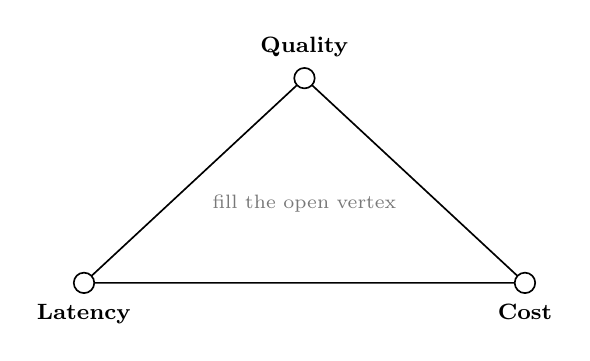
\begin{tikzpicture}[x=1mm,y=1mm,font=\footnotesize]
\coordinate (Q) at (0,26); \coordinate (L) at (-28,0); \coordinate (C) at (28,0);
\draw[line width=0.6pt] (Q)--(L)--(C)--cycle;
\foreach \p in {Q,L,C}{\draw[fill=white, line width=0.6pt] (\p) circle (1.3);}
\node[above=1.5mm of Q] {\textbf{Quality}};
\node[below=1.5mm of L] {\textbf{Latency}};
\node[below=1.5mm of C] {\textbf{Cost}};
\node[font=\scriptsize, text=rule] at (0,10) {fill the open vertex};
\end{tikzpicture}
\end{minipage}%
\begin{minipage}[t]{0.5\textwidth}
\vspace{0pt}
\hint{Quality: \rule{0.7\linewidth}{0.3pt}\newline fixed by \rule{0.3\linewidth}{0.3pt} / solved}\vspace{2mm}
\hint{Latency: \rule{0.7\linewidth}{0.3pt}\newline fixed by \rule{0.3\linewidth}{0.3pt} / solved}\vspace{2mm}
\hint{Cost: \rule{0.7\linewidth}{0.3pt}\newline fixed by \rule{0.3\linewidth}{0.3pt} / solved}\vspace{2mm}
\hint{Freshness (fourth axis): \rule{0.6\linewidth}{0.3pt}\newline \rule{0.7\linewidth}{0.3pt}}
\end{minipage}
\newpage

% ---------------- 4 Decision line and diagram
\sheettitle{Decision line}{Choose, minutes 18--21}
\hint{One boxed sentence with three parts, then the diagram drawn as its consequence with the envelope's numbers on the arrows. ``I am choosing X over Y, because the brief weights A above B, and I accept C.'' The model is a position on the quality--latency edge with a cost, not a name.}
\vspace{3mm}
\begin{tabularx}{\textwidth}{|Y|}
\hline
\textbf{I am choosing} \hfill \textbf{over} \\[26mm]
\hline
\textbf{because} \hfill \\[16mm]
\hline
\textbf{I accept} \hfill \\[16mm]
\hline
\end{tabularx}
\vspace{4mm}
\textbf{The diagram at minute fifteen}\par\hint{drawn after the decision line; every arrow carries a number from the envelope; the model is one box with its size and its cost}
\vspace{2mm}
\begin{tabularx}{\textwidth}{|Y|}
\hline
\\[108mm]
\hline
\end{tabularx}
\newpage

% ---------------- 5 Loop sheet
\sheettitle{Loop sheet}{Close the loop, minutes 35--43}
\hint{Five rows, written before the metric is read. The shipping rule goes in the second row before the test runs. The feedback row says what the model does to its own data. Harm has a measurement by group and a rollback with a clock.}
\vspace{3mm}
\begin{tabularx}{\textwidth}{L|Y}
\toprule
\textbf{Before shipping} \newline \hint{the suite by slice; the golden set; the guardrails; the time-ordered split} & \\[24mm]
\midrule
\textbf{After shipping} \newline \hint{the canary; the A/B by unit and its length; the slow read; the shipping rule, written now} & \\[24mm]
\midrule
\textbf{Silent failures} \newline \hint{nulls, lag, lost state, a drifting judge, a cache older than its TTL: what fails with no alarm} & \\[24mm]
\midrule
\textbf{Feedback} \newline \hint{what the model does to its own labels; what users or adversaries learn; how it is seen} & \\[24mm]
\midrule
\textbf{Harm and rollback} \newline \hint{errors by group; what is versioned separately; what reverts on which clock; the irreversible step} & \\[26mm]
\bottomrule
\end{tabularx}
\newpage

% ---------------- 6 Timing sheet
\sheettitle{Timing sheet}{The mock protocol, Chapter 15}
\hint{The partner holds this. Write the minute each artefact was complete and the minute the candidate first named a model. At the end the candidate writes their own guesses in the last column before seeing the sheet; the gap is the measure.}
\vspace{3mm}
\begin{tabularx}{\textwidth}{L|>{\centering\arraybackslash}p{22mm}|>{\centering\arraybackslash}p{22mm}|>{\centering\arraybackslash}p{22mm}|Y}
\toprule
\textbf{Artefact} & \textbf{Plan (45)} & \textbf{Plan (60)} & \textbf{Actual} & \textbf{Candidate's guess / notes} \\
\midrule
Brief restated & 2 & 2 & & \\[5mm]
\midrule
Objective sheet complete & 7 & 8 & & \\[5mm]
\midrule
Envelope complete & 13 & 15 & & \\[5mm]
\midrule
Binding sentence said & 15 & 17 & & \\[5mm]
\midrule
\textbf{First model named} & $\geq$ 15 & $\geq$ 17 & & \\[5mm]
\midrule
Tradeoff table and triangle & 18 & 21 & & \\[5mm]
\midrule
Decision line & 20 & 23 & & \\[5mm]
\midrule
Diagram finished & 21 & 24 & & \\[5mm]
\midrule
Mechanism worked (which?) & 35 & 36 & & \\[5mm]
\midrule
Second mechanism (60 only) & --- & 47 & & \\[5mm]
\midrule
Loop sheet started & 35 & 50 & & \\[5mm]
\midrule
Loop sheet complete & 43 & 58 & & \\[5mm]
\midrule
Close delivered & 45 & 60 & & \\[5mm]
\bottomrule
\end{tabularx}
\vspace{8mm}
\textbf{Pushes delivered and what happened}\quad\hint{conceded and priced / defended / return edge named}
\vspace{2mm}
\begin{tabularx}{\textwidth}{|Y|}
\hline
\\[22mm]
\hline
\end{tabularx}
\newpage

% ---------------- 7 Self-scoring sheet
\sheettitle{Self-scoring sheet}{The rubric of Chapter 16}
\hint{Score each row below, at or above the bar, from the anchors in Chapter 16; the partner scores separately and the two sheets are compared row by row. Mark the row that decides this brief first: if it is below the bar the design is below the bar. Note any red flag from Section 16.5 at the foot.}
\vspace{3mm}
\begin{tabularx}{\textwidth}{L|>{\centering\arraybackslash}p{14mm}|>{\centering\arraybackslash}p{14mm}|>{\centering\arraybackslash}p{14mm}|Y}
\toprule
\textbf{Row} & \textbf{Below} & \textbf{At} & \textbf{Above} & \textbf{The sentence quoted, or what was missing} \\
\midrule
Objective & & & & \\[13mm]
\midrule
Bound & & & & \\[13mm]
\midrule
Binds & & & & \\[13mm]
\midrule
Choose & & & & \\[13mm]
\midrule
Deepen \newline \hint{was it the binding part?} & & & & \\[13mm]
\midrule
Close the loop & & & & \\[13mm]
\midrule
Recovery & & & & \\[13mm]
\bottomrule
\end{tabularx}
\vspace{4mm}
\begin{tabularx}{\textwidth}{L|Y}
\toprule
\textbf{Row that decides this brief} & \\[8mm]
\midrule
\textbf{Red flags} & \\[12mm]
\midrule
\textbf{Decision} \newline \hint{hire / no hire, with the row quoted} & \\[12mm]
\bottomrule
\end{tabularx}
\end{document}
